\documentclass[letter,10pt]{article}
\usepackage{authblk}
\usepackage{geometry}
\geometry{margin=.75in}
\usepackage{graphicx}
\graphicspath{ {./images/} }
\usepackage{enumitem}
\usepackage{amsmath}
\usepackage{amssymb}
%\usepackage{biblatex}
\usepackage[backend=biber]{biblatex}
\addbibresource{references.bib}

\begin{document}
\title{The Hollow Heap Data Structure: An Introduction, Run-Time Analysis, and Comparison to the Fibonacci Heap}
\author{Alisha Sprinkle and Courtney Dixon}
%\affil{CS 5110 - The Design and Analysis of Algorithms}
\date{December 8, 2019}
\maketitle

\section{Abstract}
\qquad Hollow Heaps were introduced by Hansen, Kaplan, Tarjan, and Zwick in 2015. This data structure performs operations with the same amortized efficiency as the Fibonacci Heap introduced by Tarjan and Fredman. Hollow Heaps perform all operations characteristic of a heap, however, Hollow Heaps use lazy deletion and a directed acyclic graph rather than trees. The goal of this paper is to explain the Hollow Heap data structure precisely, analyze the amortized running time of the data structure, implement the data structure in Java, and compare the efficiency of Hollow Heaps to the renown Fibonacci Heap data structure.

\section{Hollow Heap: the data structure}
``Clearly explain the data structure"\\

\qquad A Hollow Heap is a heap-ordered data structure. Therefore, a Hollow Heap maintains the heap property; the key of Node a is less than or equal to the key of Node b for every directed arc(a,b) in the structure where Node a is the parent of Node b. The typical properties of nodes still hold. A node that does not have a parent is a root and a node that does not have any children is a leaf. The root has the minimum key in the Hollow Heap.\\\\
Hollow Heaps are just as efficient as Fibonacci Heaps. All the operations of a heap, excluding two, take $O(1)$ time in the worst case and amortized with Hollow Heaps. The two heap operations that take longer than constant time are \textit{delete} and \textit{deleteMin}, which each take $O(\log n)$ amortized time with Hollow Heaps. The \textit{decreaseKey} operation in Hollow Heaps uses lazy deletion and reinsertion. Other heaps use a tree or set of trees, but Hollow Heaps use a directed acyclic graph (dag) instead. A Hollow Heap is made up of nodes that hold items and not the typical nodes that are items. The node structure is depicted in the image below.
\begin{center}
	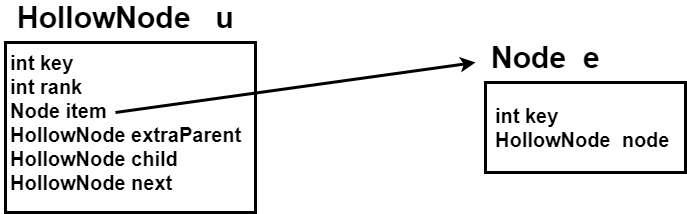
\includegraphics[scale=.5]{one.png}
\end{center}
The authors presented three variants of the Hollow Heap data structure: Multi-root, One-root, and Two-parent. The focus in this paper is the Two-Parent Hollow Heap.  

\subsection{Methods}
%\begin{enumerate}
%\begin{enumerate}[label=(\alph*)]
%\renewcommand{\labelitemi}{$\blacksquare$}
%\renewcommand\labelitemi{$\square$}
\begin{itemize}
	\item makeHeap()
	\item findMin(HollowHeap h)
	\item insert(Node e, int key, HollowHeap h)	
	\item deleteMin(HollowHeap h)
	\item meld(HollowNode g, HollowHeap h)	
	\item decreaseKey(HollowNode e, int key, HollowHeap h)
	\item delete(HollowNode e, HollowHeap h)
	\item makeNode(wNode e, int key)
	\item link(HollowNode v, HollowNode w)
	\item addChild(HollowNode v, HollowNode w)	
	\item doRankedLinks(HollowNode u)
	\item doUnrankedLinks()
	
\end{itemize} 

\section{Amortized Analysis via the Accounting Method}
``Amortized Analysis via Accounting Method"
\begin{center}
	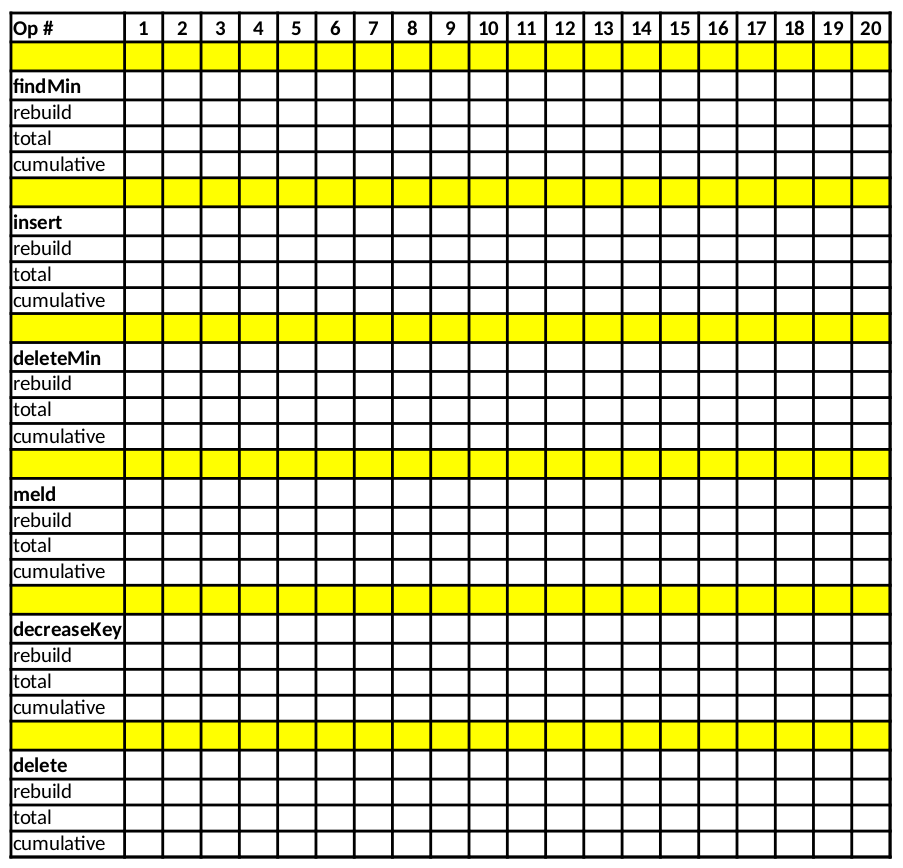
\includegraphics[width=\textwidth,height=\textheight]{accounting.png}
\end{center}

\section{Hollow Heap Implementation} 
The authors presented three variants of the Hollow Heap data structure: Multi-root, One-root, and Two-parent. Our implementation is of Two-Parent Hollow Heaps. Our programs are written in the Java programming language. The UML diagram below is for the Hollow Heap class. All other UML diagrams can be found in the figures section of this paper. 

\section{Hollow versus Fibonacci: A Comparison}
``Compare the two data structures in terms of practical efficiency"
\subsection{Similarities}
\begin{enumerate}
    \item heap operations in $O(1)$ and $O(\log n)$
    \item simple to implement
    \item
\end{enumerate}

\subsection{Dissimilarities}
\begin{enumerate}
    \item Tree(s) versus Dag
    \item no cascading cuts
    \item 
\end{enumerate}

\section{Figures}
\begin{center}
	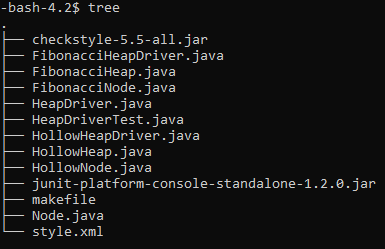
\includegraphics[]{tree.png}\\
	Figure : Directory Tree
\end{center}
%\phantom{helloworld}\\
\medskip
\begin{center}
	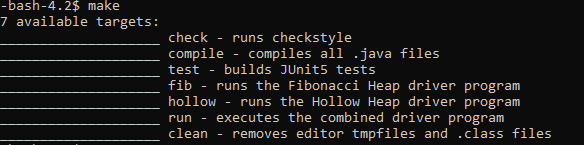
\includegraphics[]{make.png}\\
	Figure :  Makefile Targets
\end{center}
%\begin{center}
%	\includegraphics[]{.png}
%\end{center}

\newpage
\nocite{*}
\printbibliography

\end{document}

